\chapter{Design and Implementation} %  Design Principles and Architecture
%TODO add chapter introduction

% - 5-10 pages
% - goal: fellow student understands content and would be able to more or less reproduce work
% - legitimate chosen approach
% - develop own ideas, trace them to existing theories
% - analysis and development
% - why was the approach (algorithm/technique/...) chosen and how does it work
% - show how concepts from theory are applied
% - test setup and achieved results

% possible steps:
% - requirement study
% - analysis / design -> UML, interaction, behavioural model, basic algorithms/methods, detailed description of models and their interactions (class/sequence diagrams)
% - manual, how to use program/device
% - system development and implementation

% ---

% considerations:
% - ipv6 not 100 percent necessary, but would be good
% - easy to learn
% - easy to adapt (to counterpart-interface updates) -> plug-in system?
% - tosca-orchestrator:
%   - 4.3ff of \url{http://docs.oasis-open.org/tosca/TOSCA-Instance-Model/v1.0/csd01/TOSCA-Instance-Model-v1.0-csd01.html#_Toc500843787}
%     "orchestrators manage the state of nodes and transitions them from state to state. This notion of state is somewhat artificial in that the orchestrator assumes a stable state is reached after an operation executes [...] without error"
%     "an error results in an undefined state" (no automatic rollback defined in tosca)
%     "orchestration states are only valid during orchestration. [...] the orchestrator or the imperative workflow [...] must decide the current state of all nodes in the topology.
%     "[...] event stream can be maintained for the life of a deployment [...]"
%     "As nodes are transitioned through their states, a subset of attributes and relationships may be defined. [...] This requires that in general TOSCA implies semantics such that not all attributes would be available in a given state."
%     "Nodes are only visible when they have a state defined (i.e. the orchestrator is dealing with their lifecycle)"
%     "node attributes are only defined for the stable states"
%     "node relationships are always navigable when the source and target node exists"
%     "[...] state is never updated outside an orchestration. [...] no way to propagate state changes from the node to the orchestrator and nodes don't have a state attribute."
%       -> no state file!
%     "Nodes can update their attributes with no specific guarantees in terms of precision or accuracy"

\section{Requirements}
The orchestrator should understand \gls{toscaacr}, extensions from it and should be able to provision bare-metal machines. Not only is it possible to split this into subtasks, but it makes sense as well. By doing so, the modules can be developed and updated one after another, in parallel if necessary and at a later point even interchanged with other implementations. In order to slice the application into reasonable packages, their domains should not overlap, and their external interface as small as possible.
\newline
To achieve that goal, the application workflow needs to be analyzed:
\newline
At the beginning, the \gls{csaracr} files, its content and the \gls{yamlacr} structure of the content needs to be parsed and validated. This includes handing down properties of both type-from-type and template-from-type derivations, as well as enabling (namespaced) imports.
Then, the orchestrator must be able to wake machines with \gls{wolacr}.
After a machine is powered on, it attempts to boot over network.
Therefore, the orchestrator has to manipulate an external or internal (as in \textquote{integrated in the orchestration software}) \gls{dhcpacr} server.
In order to provide the orchestrator with the necessary information about the machine, it makes sense to use a live-\gls{osacr} that does not need to be installed, but can be booted directly. Optimally, it should be relatively small, since its transferred via network, boot fast, and somehow provide the orchestrator with information about the underlying hardware like its RAM-size.
The last step is then running commands on the machine like installing a package or copying files to it. Optimally, the user should be informed on what is currently going on during the whole process.
\newline
Figure \ref{image:workflow} shows the whole workflow in an interaction overview diagram.

\begin{figure}[H]
  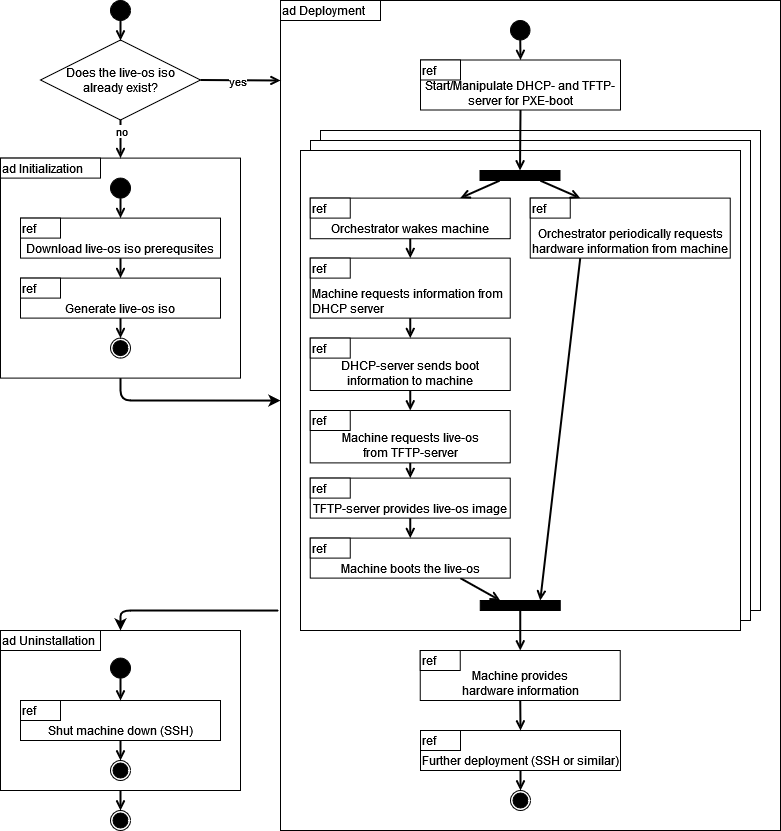
\includegraphics[width=14cm]{workflow}
  \centering
  \caption{UML interaction overview diagram describing the application workflow}
  \label{image:workflow}
\end{figure}

\section{Architecture}
To diminish the limitations of a web-based approach for the orchestrator like the hogging of resources even during idle times, the goal is to have one or many libraries, and a commandline-based wrapper around it.
\newline
As described above, the tasks of the orchestrator can (and should) be split into different steps. For example the wake-on-lan module and the \gls{dhcpacr} server have nothing in common except both being invoked from the orchestrator whenever they are needed.
\newline
The executable has at least three subcommands; One for initialization, where the live-\gls{osacr} image is generated and the \gls{dhcpacr} server is prepared. And a second where the actual deployment happens. Last but not least, an uninstallation subcommand is needed to reverse the deployment.
\newline
The following chapters describe, how the domains within those subcommands are sliced in order to have different modules for the different domains.

\section{Packages}
Most of the packages described in the following chapters strongly relate to the steps described in figure \ref{image:workflow}. They are described in the order they are invoked during both the initialization and deployment subcommands. A summary of interactions and dependencies is shown in the package diagram in figure \ref{image:packages} below.

\begin{figure}[H]
  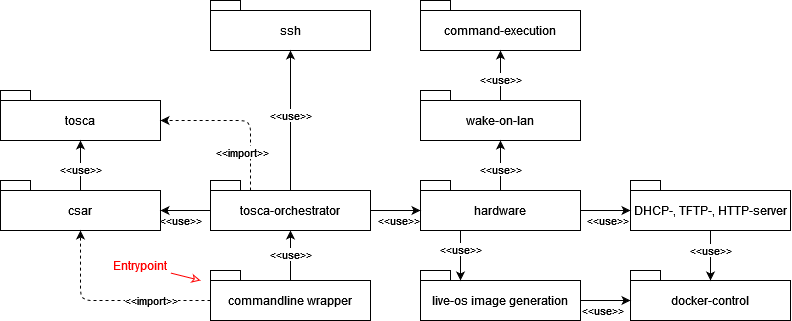
\includegraphics[width=14cm]{packages}
  \centering
  \caption{UML package diagram describing how the packages are related to each other}
  \label{image:packages}
\end{figure}

\subsection{TOSCA}
In order to be able to implement a library for the \gls{toscaacr} standard, it is necessary to work through both the original specification and the Simple-Profile extension counterpart, since both are meant to work together. Important information is sometimes distributed over both specifications, so to fully understand it, this is necessary. Additionally, preexisting libraries for the chosen programming language might exist. In case of this thesis' reference implementation Golang is the language of choice. Sadly, most of the larger libraries are based on one another or unfinished, and the most complete of them was severly outdated \cite{github_toscalib_forks}.
\newline
In order to support the latest version of the specification, and to be able to easily extend it if necessary, a complete reimplementation of the \gls{toscaacr} library was created. It is strongly influenced by the largest but outdated one, but is more complete. Only with the already described line-by-line read-through of both specifications it is possible to gather enough information about the standard and all its features.
\newline
With the new library, it is possible to parse any Service Types, Templates, and Topologies.
In addition to parsing them and creating Go-native structures out of them, basic functions like \textquote{get\_input} and \textquote{get\_attribute} or validation of elements, it is limited to one implementation type, Bash, while the specification states that Python should be supported as well. This is due to the proof-of-concept nature of this thesis. Sadly, there are several occasions in the specifications, where it is unclear or simply incomplete. These cases are mostly about edge cases and were not required for the proof-of-concept this thesis tries to achieve. Therefore, they were left out of the implementation. Inconsistencies will be covered in the chapter \textquote{Analysis}.
\newline
Because the basic TOSCA specification describes how to work with extensions like the TOSCA Simple Profile, it is possible to implement such imports, references, and relations as well. This means, the implemented TOSCA library (called package in Golang context) is fully compatible with the TOSCA Simple Profile and all other extensions.
\newline
The package is also meant to solve the type derivation, resolve imports, namespacing and validate all of them.

%TODO add TOSCA processor, orchestrator etc definitions, and what is fulfilled or not

% describe public functions

\subsection{CSAR}
After the TOSCA package was able to parse the contents of files, the last chapter of the specification was implemented as a seperate package. It contains information about how to pack multiple artifacts like \gls{osacr}-images, definition-, or other required files together into one CSAR file. The file is basically a zip-archive, but the contents need to follow a certain schema. For example there are three places where metadata like version and name can be placed. If they are not found there, the whole file is invalid.
\newline
The reason behind this seperation are the still very different domains: The \gls{toscaacr} package parses file contents and provides Go-native types, while the \gls{csaracr} package is more about accessing files, checking for their existance and making it possible for the \gls{toscaacr} package to parse its content.
\newline
This package depends on the earlier one, but has a function that takes a file-/folderpath as input and returns the fully parsed \gls{toscaacr} topology with fully derived templates (meaning all properties form the origin types are included already).

%TODO describe public functions

\subsection{Command-execution}
In order to run Bash commands from the application itself and retrieve the outputs, it makes sense to build a complete package around command execution. Its can later be extended with a Python implementation, so the application is fully compatible to the \gls{toscaacr} specification.
%TODO add more

\subsection{Docker control}
It is clear , that some kind of DHCP- and TFTP-server is required. And those require an easily repeatable setup. As in most such cases, this can be solved with docker. But because the goal of this thesis is to bring all required bits together, it is necessary to create the docker images, start containers (with parameters like volumes and forwarded ports), as well as stopping and removing the containers when they are not needed anymore (for example when provisioning is finished).
\newline
The official docker binary (for Linux) is created in Golang as well, and the software is open source. Docker even provides an SDK for other developers to integrate communication with the docker engine into their applications.
Sadly, the documentation is sparse and the few examples shown along the SDK are often not enough to get even seemingly easy things like container stopping to work. For this particular example it is necessary to add the container stopping and removal twice: Once, when the application terminates successfully, as the container fulfilled its job and isn't needed any more. And a second time, when the application terminates due to an error somewhere else, and the default termination does not happen. Even \textquote{deferring} the container termination did not work. Only when the SIGTERM interrupt is \textquote{manually} listended for and a function is implemented to remove the container in such a case, the removal is successfull in all cases.
\newline
Another obstacle is the retrieval of live logs during the container livecycle and embed the retrieved output in the logs of the wrapping application. It can be solved by creating a buffered streamreader, which polls periodically for contained linebreaks.
\newline
As the application is now able to handle docker containers to provide repeatable setup of the DHCP- and TFTP-server, the next step is to implement a repeatable way of a live-\gls{osacr} image generation.

\subsection{Live-OS image generation}
In order to be able to create the iso-file from scratch, only one requirement should exists: a working internet connection. Optimally, a generic image is downloaded and then modified to serve the special use case of publishing information about the underlying hardware. Since tiny linux images should be relatively common in times of Internet-of-Things and Raspberry Pis, this was first estimated to be an easy task.
\newline
As one can imagine, it turned out differently. The first linux distribution tested during the implementation phase was \textquote{Minimal Linux Live}.
%TODO add notes about tests with different operating systems (size, speed, repeatable, webserver-capable)
% start with MLL
% then alpine
% then ubuntu
% then debian in more detail

% why web-server, how to add additional information about the hardware

\subsection{DHCP-, TFTP-, HTTP-server}
docker container, ports, variable config vs fixed config

\subsection{Wake-on-lan}
actual wol vs simulated wol for hypervisors

\subsection{SSH}
key-generation, variable key path, key placement on servers
\newline
actual command execution and feedback returning

\subsection{TOSCA hardware extension}
types, topology, tests
